\documentclass{article}
\usepackage{graphicx} % Required for inserting images
\usepackage{authblk} % For author affiliations
\usepackage{hyperref} % For hyperlinks
\usepackage[margin=1in]{geometry} % Standard margins
\usepackage{natbib} % For bibliography management
\usepackage{enumitem} % For customising lists

\newlist{tree}{itemize}{10}
\setlist[tree]{label=-}
\setlistdepth{10} 


\title{Integrating Multiple Data Sources in Infectious Disease Modelling: Best Practices and Implementation}

\author[1]{Sam Abbott}
\author[2]{Xiahui Li}
\author[3]{Punya Alahakoon}
\author[4]{Dhorasso Junior Temfack Nguefack}
\author[5]{Johannes Bracher}
\author[6]{Felix Günther}
\author[7]{@working-group-members}
\author[8]{@workshop-participants}
\author[9]{Mircea T. Sofonea}
\author[10]{Michael Plank}
\author[11]{Anne Presanis\thanks{Joint last authors}}
\author[12]{Anne Cori$^*$}

\affil[1]{London School of Hygiene \& Tropical Medicine}
\affil[2]{University of St Andrews}
\affil[3]{University of Oxford}
\affil[4]{Trinity College Dublin}
\affil[5]{Karlsruhe Institute of Technology}
\affil[6]{Robert Koch Institute}
\affil[7]{@working-group-affiliations}
\affil[8]{@workshop-participant-affiliations}
\affil[9]{University of Montpellier, France}
\affil[10]{University of Canterbury, New Zealand}
\affil[11]{MRC Biostatistics Unit, University of Cambridge}
\affil[12]{Imperial College London}

% Note: Author order is provisional and subject to change

\date{\today}

\begin{document}

\maketitle

\begin{abstract}
Infectious disease modelling increasingly relies on integrating multiple data sources to improve parameter estimation and reduce uncertainty.
However, practitioners face complex choices about how to combine diverse data streams, from full joint modelling to modular approaches that fit sub-models separately before integration.
This paper provides a comprehensive framework for integrating multiple data sources in infectious disease modelling, with transmission intensity estimation as a key exemplar.
We review data source characteristics, present a structured workflow for model development, and compare integration approaches including joint modelling, evidence synthesis methods, and ensemble techniques.
Through worked case studies progressing from single data sources to multi-stream integration, we demonstrate how different data types provide complementary information for estimating parameters such as time-varying reproduction numbers and overdispersion.
We discuss computational considerations, model validation strategies, and practical implementation challenges.
Our modular framework emphasises parsimony, interpretability, and systematic assessment of conflict between data sources.
This work addresses a critical gap in the literature by providing practical guidance for infectious disease modellers on data integration choices, supported by reproducible examples and decision-making frameworks.
\end{abstract}

\section{Introduction}
% Lead: Sam Abbott

% Paragraph 1: Motivation and Context
Infectious disease modelling increasingly relies on integrating multiple data sources to improve parameter estimation, reduce uncertainty, and provide more robust evidence for public health decision making [@placeholder].
Recent outbreaks including COVID-19, mpox, and Ebola have highlighted both the potential value and practical challenges of combining diverse data streams such as case reports, deaths, hospitalisations, genomic sequences, wastewater surveillance, and serological surveys [@placeholder].
Single data sources often provide limited or biased information about key epidemiological parameters, whilst multiple sources can offer complementary perspectives that improve model accuracy and reliability [@placeholder].
However, practitioners face complex methodological choices about how to combine these data streams effectively.

% Paragraph 2: Current Approaches
Current approaches to multi-source integration broadly fall into two categories: pipeline methods that fit separate models to individual data sources before combining estimates, and joint modelling approaches that simultaneously fit all data sources within a unified statistical framework [@placeholder].
Pipeline approaches offer computational efficiency and modular development but may propagate errors and fail to capture dependencies between data sources [@placeholder].
Joint modelling can provide more principled uncertainty quantification and better parameter identifiability, but often requires substantial computational resources and model complexity [@placeholder].
Existing guidance for practitioners is fragmented across methodological literature, with limited practical frameworks for navigating integration choices systematically [@placeholder].

% Paragraph 3: Paper Scope and Contribution
This paper provides a framework for integrating multiple data sources in infectious disease modelling, with practical implementation as the primary focus.
We use transmission intensity estimation—specifically time-varying reproduction numbers and overdispersion parameters—as a case study to demonstrate broader principles applicable across infectious disease modelling contexts.
Our approach encourages iterative model building, allowing practitioners to systematically assess the value of additional data sources while maintaining interpretability and computational tractability.
The framework addresses critical gaps in existing literature by providing domain-specific guidance and signposting to more generic resources for integration choices, validation strategies, and conflict resolution between data sources.

% Paragraph 4: Paper Structure
We first review data source characteristics and present a structured iterative workflow for model development that progresses from research question definition through process and observation DAG development to integration method selection.
We then compare integration approaches from full joint modelling to modular ensemble methods.
Three worked case studies demonstrate progressive complexity: single-source baselines, two-source integration, and multi-stream applications incorporating individual-level data.
Each case study follows our iterative workflow, demonstrating how DAG-based model development guides data integration decisions.

\section{Data Sources and Characteristics}
% Lead: Punya Alahakoon

We conducted a survey of workshop participants to systematically evaluate different data sources for infectious disease modelling.
This tool helps practitioners rate different data sources on quality, timeliness, and usefulness for modelling SARS-CoV-2.
By pooling expert opinions, we have created visual comparisons showing trade-offs between different data types, making it easier to decide which data to use when estimating transmissibility and identifying when different sources might conflict.

Participants evaluated candidate datasets across six main categories: basic metadata, scope, resolution, data quality, data utility, and practical considerations.
For each subcategory, experts assigned values between 0 and 5, selected appropriate categories, or provided free text responses.
We harmonised and ensembled these expert assessments to create overview tables and data analysis.

% TODO: Present survey results and expert consensus
% TODO: Create comprehensive table of data characteristics  
% TODO: Discuss taxonomy of data sources in infectious disease surveillance
% TODO: Analyse information content and complementarity
% TODO: Address preprocessing and standardisation requirements

\section{Workflow}
% Lead: Sam Abbott

\subsection{Overview}

We recommend following a structured, iterative workflow for multi-data source modelling (Figure~\ref{fig:workflow}).

\begin{figure}[htbp]
    \centering
    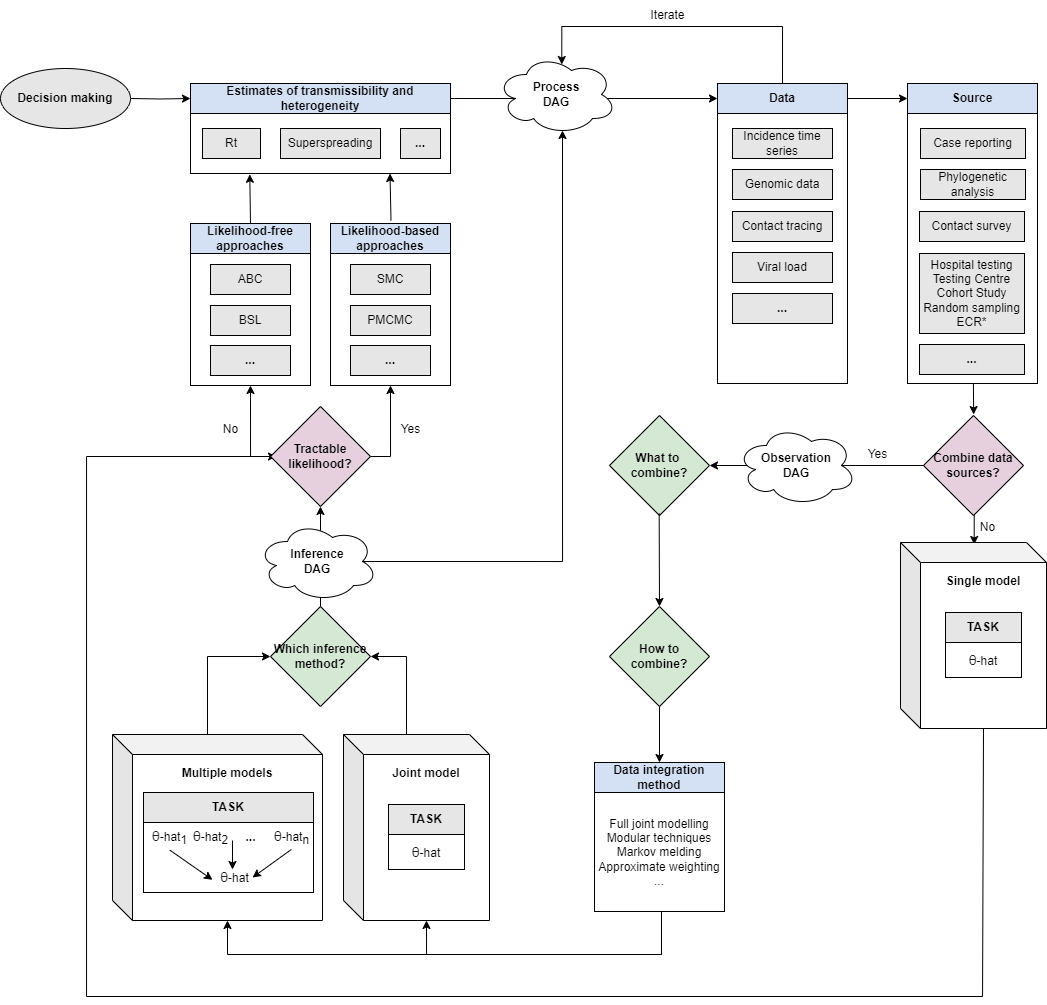
\includegraphics[width=\textwidth]{figures/workflow-schematic.png}
    \caption{Recommended workflow for integrating multiple data sources in infectious disease modelling. Begin by defining research questions and target estimands, proceed through iterative development of process and observation DAGs, and follow critical decisions about data integration and inference methods.}
    \label{fig:workflow}
\end{figure}
Start with a clear research question—such as estimating transmission intensity—and use systematic model development through directed acyclic graphs (DAGs) with iterative refinement.
We advocate this approach because it makes modelling choices transparent, assumptions explicit, and allows systematic assessment of additional data sources.

We recommend beginning with \textbf{decision making}: clearly define your research question and target estimands (e.g., time-varying reproduction number, overdispersion parameters).
Next, develop a \textbf{process DAG} representing the underlying epidemiological process, iterating on this representation as understanding develops.
Map available \textbf{data sources} to your process model, such as incidence time series, genomic data, contact tracing, viral load measurements, and serological surveys.
For each data source, develop an \textbf{observation DAG} linking the underlying process to observed data through measurement models and reporting mechanisms.
Different data sources may also impact your \textbf{process DAG} assumptions, such as if you can collapse your approach from individual-level to population-level.

Once you have developed your process and observation DAGs, proceed to \textbf{model specification and validation}, including prior specification, parameter identifiability assessment, and diagnostic approaches.
You then face the key decisions: \textbf{"What to combine?"} and \textbf{"How to combine?"}
If combining multiple sources is not beneficial or feasible, you can proceed to single-source modelling and combination of estimates.
If integration is warranted, select among data integration methods including full joint modelling, modular techniques, Markov melding, or approximate weighting approaches.
Finally, fit your model and evaluate its performance through posterior predictive validation and sensitivity analysis.

In the following sections, we will discuss each of these steps in more detail.

\subsection{Research Question and Target Estimands}
% TODO: Defining clear research objectives
% TODO: Specifying target parameters and estimands
% TODO: Connecting questions to policy needs
% TODO: Setting scope and boundaries

\subsection{Process DAG Development}
% TODO: Representing epidemiological processes
% TODO: Causal relationships and assumptions
% TODO: Iterative refinement based on understanding
% TODO: Incorporating biological mechanisms

\subsection{Data Source Mapping}
% TODO: Cataloguing available data streams
% TODO: Assessing data characteristics and biases
% TODO: Linking data to process components
% TODO: Evaluating complementarity and redundancy

\subsection{Iterate on the Process DAG}

%TODO: based on available data sources and the original process DAG may need to iterate
%TODO: An example is the need for individual level modelling for certain data sources which might impact the construction of the process DAG.

\subsection{Observation DAG Construction}
% TODO: Measurement models and reporting processes
% TODO: Delays and missing data mechanisms
% TODO: Linking latent processes to observations
% TODO: Accounting for data collection protocols

\subsection{Model Specification and Validation}\label{sec:spec-validate}
% TODO: Bayesian workflow principles
% TODO: Prior specification and prior predictive checks
% TODO: Parameter identifiability assessment
% TODO: Model criticism and diagnostic approaches
% TODO: Posterior predictive validation
% TODO: Cross-validation strategies
% TODO: Sensitivity analysis frameworks

\subsection{Data Integration Choices}
% Lead: Anne Presanis

%Consideration: How do we clearly split here between combined and individual approaches? What does that structure look like? How do we connect this question to fitting choices which in practice are important?
%Consideration: What parts of this (sub models etc etc are part of specification and validation. How does that interaction work?
%Consideration: There might be an ideal DAG structure but in practice need to approximate for fitting. I.E want to use NUTs so can't have latent discrete parameters etc...

Attempt at tree of choices:
\begin{tree}
    \item Are you combining alternative/competing models from different groups?
    \begin{tree}
        \item Yes
        \begin{tree}
            \item How are the results from each available?
            \begin{tree}
                \item As point estimate and confidence/credible interval
                \begin{tree}
                    \item Do you trust the alternatives equally?
                    \begin{tree}
                        \item Yes
                        \begin{tree}
                            \item $\Rightarrow$ standard meta-analysis
                        \end{tree}
                        \item No
                        \begin{tree}
                            \item $\Rightarrow$ weighted meta-analysis, weighted by precision
                            \item $\Rightarrow$ or weighted by other criteria, e.g. prediction accuracy (ensembling)
                        \end{tree}
                    \end{tree}
                \end{tree}
                \item As posterior samples or analytic posterior distribution
                \begin{tree}
                    \item Do you trust the alternatives equally?
                    \begin{tree}
                        \item Yes
                        \item No
                    \end{tree}
                \end{tree}
            \end{tree}
        \end{tree}
        \item No
        \begin{tree}
        \item Are your sub-models independent conditional on their common parameters?
        \begin{tree}
            \item Yes
            \begin{tree}
                \item Do 
            \end{tree}
            \item No
        \end{tree}
        \end{tree}
    \end{tree}
\end{tree}


First stab outline 27/05
\begin{itemize}
    \item Different possible choices for integrating/ensembling inference from multiple data sources
    \begin{itemize}
        \item Full joint model fitted, regardless of whether you have already fitted separate sub-models
        \item Conditionally independent sub-models each fitted separately, then integrated
        \begin{itemize}
            \item Meta-analysis of separate estimates
            \item Weighted averaging / ensembling
            \item Markov melding
        \end{itemize}
    \end{itemize}
    \item Depends on whether you are starting from scratch, from an existing model for one data source to which you want to add others, or whether you have multiple alternative sets of existing inferences from different data sources that you want to combine
    \item General principle that modular model building (De Angelis et al, 2015; Birrell et al, 2018; Goudie et al, 2019; De Angelis \& Presanis, 2019; Gelman et al, 2020; Nicholson et al, 2022, Liu \& Goudie, 2025) is preferable, since:
    \begin{itemize}
        \item Easier to understand lack of fit, model misspecification or convergence issues from simpler sub-models individually
        \item Occam's razor - principle of parsimony, start from simplest model and build complexity up only as far as needed
        \item Adding sub-models in one at a time allows for assessment of consistency/conflict between sub-models sequentially
        \item Computational efficiency - rather than fitting full joint models after fitting the sub-models, use the posterior samples from the sub-models to obtain your full joint model (melding or ?)
    \end{itemize}
    \item Choice of likelihood function (or other objective function) and fitting choices (\ref{sec:fitting}) therefore depends on options above on where you are starting from (existing models/sub-models or from scratch)
    \item And model development is a cycle of model building and model criticism
    \begin{itemize}
        \item extension of model validation in \ref{sec:spec-validate} to multiple data sources setting
        \item detection/measurement of conflict not only between prior and data, but between data and data, or partitions of the DAG (modules) comprising different combinations of prior and data, i.e. posterior-posterior comparisons
        %\item TODO: conflict references from Fuming's literature review
    \end{itemize}
\end{itemize}

% TODO: Add practical examples of each approach
% TODO: Include decision framework for choosing integration method

\subsection{Fitting Choices}\label{sec:fitting}
% Lead: Anne Presanis, with Dhorasso and Xiahui

\subsubsection{Tools for Tractable Likelihood Functions}
% TODO: MCMC and its variants for joint models
% TODO: Particle MCMC (pMCMC) for state-space formulations
% TODO: Sequential Monte Carlo (SMC) approaches
% TODO: Variational inference (VI) and INLA for specific model classes

\subsubsection{Tools for Intractable Likelihood Functions}
% TODO: Approximate Bayesian Computation (ABC-MCMC, ABC-SMC)
% TODO: ABC with history matching
% TODO: Bayesian Synthetic Likelihood (BSL)
% TODO: Simulation-based inference approaches

\subsubsection{Selecting the Right Tool}
% TODO: Trade-offs between computational complexity, accuracy, bias
% TODO: Interpretability and implementation ease considerations
% TODO: Decision-making frameworks for method selection

\subsubsection{Practical Implementation}
% Lead: Sam Abbott
% TODO: Software implementations and availability
% TODO: Diagnostic tools and convergence assessment
% TODO: Computational resource requirements
% TODO: Reference to inference subpanel workflow figure

\section{Case Studies}
% Lead: Anne Cori

\subsection{Overview}

We demonstrate our iterative workflow through four progressive case studies, each building complexity whilst showing different integration choices and methodological considerations.
All case studies share common estimands—time-varying reproduction number (Rt) and overdispersion parameter (k)—using SARS-CoV-2 outbreak data to leverage expert survey evidence on data source characteristics.
Each case study follows our complete workflow framework, demonstrating how different data sources enable answering questions that would require strong assumptions with other sources alone.

The progression illustrates key principles: deaths eliminate reporting fraction assumptions that plague case-only analyses; wastewater eliminates testing bias inherent in symptomatic surveillance; individual-level data enables direct overdispersion estimation without distributional assumptions.
Implementation choices reflect practical considerations including available expertise, computational resources, and model complexity trade-offs, whilst generally favouring efficient methods like NUTS where applicable.

\subsection{Case Study 0: Single-Source Baseline (Cases Only)}

\textbf{Research Question:} What is Rt during this outbreak period using case incidence alone?

\textbf{Workflow Demonstration:}
\begin{enumerate}
    \item \textbf{Process DAG:} Simple renewal equation linking Rt to case incidence through generation time distribution, incorporating overdispersion via negative binomial model
    \item \textbf{Data Source Mapping:} Case incidence time series selected based on expert survey ratings showing high timeliness but moderate precision due to testing policy effects
    \item \textbf{Observation DAG:} Reporting delays, underascertainment fraction, weekend reporting effects
    \item \textbf{Integration Choice:} Single source (no integration required)
    \item \textbf{Implementation:} NUTS sampling of renewal equation with negative binomial observation model, chosen for computational efficiency and robust performance
\end{enumerate}

\textbf{Key Limitation:} Establishes baseline uncertainty but requires strong assumptions about generation time distribution and reporting fraction, highlighting assumption-dependent limitations that motivate multi-source approaches.

\subsection{Case Study 1: Two-Source Integration (Cases + Deaths)}

\textbf{Research Question:} How does adding death data improve Rt estimation and reduce assumption dependence?

\textbf{Workflow Demonstration:}
\begin{enumerate}
    \item \textbf{Process DAG Iteration:} Extend transmission process to include infection-to-death pathway with delay distribution
    \item \textbf{Data Source Mapping:} Expert survey shows deaths have higher reporting delays but lower noise and less policy dependence than cases
    \item \textbf{Observation DAG:} Different reporting mechanisms for cases and deaths, with longer delays for death registration
    \item \textbf{Integration Choice Comparison:} 
        \begin{itemize}
            \item \textbf{Approach A:} Joint model with shared Rt parameter
            \item \textbf{Approach B:} Separate estimates combined via weighted ensemble
        \end{itemize}
    \item \textbf{Implementation:} Particle MCMC for joint model due to state-space formulation complexity; NUTS for separate models followed by Markov melding
\end{enumerate}

\textbf{Key Insight:} Deaths enable estimation without assuming reporting fraction but require death delay distribution assumptions, demonstrating how additional data sources shift rather than eliminate modelling assumptions.

\subsection{Case Study 2: Three-Source Integration (Cases + Deaths + Wastewater)}

\textbf{Research Question:} How do we handle conflicting signals between data sources and incorporate complex observation processes?

\textbf{Workflow Demonstration:}
\begin{enumerate}
    \item \textbf{Process DAG Iteration:} Add viral shedding pathway from infections to wastewater concentration
    \item \textbf{Data Source Mapping:} Wastewater offers population-level signal independent of testing bias, with moderate timeliness but requiring environmental expertise
    \item \textbf{Observation DAG:} Complex shedding model incorporating individual-level variation, catchment population dynamics, environmental degradation
    \item \textbf{Integration Choice:} Modular approach with sequential consistency assessment to detect and resolve data source conflicts
    \item \textbf{Implementation:} ABC-SMC for wastewater sub-model due to likelihood intractability, reflecting available environmental modelling expertise; NUTS for case/death models
\end{enumerate}

\textbf{Key Insight:} Wastewater enables trend detection independent of testing policy but requires environmental and shedding assumptions, whilst modular approach facilitates conflict detection between data sources.

\subsection{Case Study 3: Individual-Level Data (Cases + Transmission Pairs)}

\textbf{Research Question:} How does individual-level data improve overdispersion estimation and change modelling assumptions?

\textbf{Workflow Demonstration:}
\begin{enumerate}
    \item \textbf{Process DAG Transformation:} Shift from population-level renewal equation to individual-level transmission process with explicit contact structure
    \item \textbf{Data Source Mapping:} Contact tracing provides transmission pairs with direct overdispersion information, contingent on tracing system quality
    \item \textbf{Observation DAG:} Observation probability for transmission pairs, contact tracing coverage and delay effects
    \item \textbf{Integration Choice:} Hierarchical model linking individual transmission events to population-level reproduction number
    \item \textbf{Implementation:} NUTS with data augmentation for unobserved transmissions, chosen for efficient handling of discrete latent variables
\end{enumerate}

\textbf{Key Insight:} Individual-level data enables direct overdispersion estimation without distributional assumptions but requires contact tracing completeness assumptions, demonstrating how data granularity can fundamentally change model structure and inference requirements.

\section{Discussion}

\subsection{Summary}

We have presented a framework for integrating multiple data sources in infectious disease modelling that emphasises practical implementation through a structured, iterative workflow.
Our approach combines systematic model development using directed acyclic graphs with modular integration strategies that prioritise parsimony, interpretability, and explicit assessment of data source conflict.
The framework progresses from clear research question definition through process and observation DAG development to informed choices about integration methods, supported by expert survey evidence on data source characteristics and worked case studies demonstrating progressive complexity.
Key contributions include the structured workflow that makes modelling assumptions transparent, the expert consensus on data source trade-offs that guides selection decisions, and practical guidance that bridges the gap between methodological advances and real-world implementation challenges.
Our modular approach incentives building complexity incrementally, allowing practitioners to assess the value of additional data sources systematically whilst maintaining computational tractability and model interpretability.

\subsection{Strengths and Limitations}
% TODO: Strengths: Modular framework, practical focus, worked examples
% TODO: Strengths: Integration of diverse methodological approaches
% TODO: Strengths: Expert survey and empirical evidence base
% TODO: Limitations: Model selection and validation challenges
% TODO: Limitations: Dependence on data quality and availability
% TODO: Limitations: Computational considerations and scalability

\subsection{Comparison with Existing Literature}
% TODO: Position relative to pipeline vs joint modelling literature
% TODO: Relationship to evidence synthesis and meta-analysis methods
% TODO: Comparison with ensemble forecasting approaches
% TODO: Distinguish from existing reviews and methodological papers
% TODO: Compare with other multi-source integration frameworks

\subsection{Outstanding Challenges and Future Directions}
% TODO: Real-time implementation constraints and solutions
% TODO: Computational scalability for large-scale integration
% TODO: Methodological gaps in current approaches
% TODO: Emerging data sources and integration needs
% TODO: Community standards and best practices
% TODO: Research priorities and next steps

\section{Conclusions}

Integrating multiple data sources offers substantial benefits for infectious disease modelling, but requires careful consideration of trade-offs between information gain, computational complexity, and interpretability.
Our framework provides infectious disease modellers with practical tools for navigating these choices through structured workflows, expert consensus on data characteristics, and demonstrated case studies that progress from single-source baselines to complex multi-stream integration.
The modular approach we advocate offers a pragmatic path forward that balances methodological rigor with practical considerations.
By making modelling assumptions explicit through DAG-based development and providing clear guidance on integration method selection, this framework enables more transparent, reproducible, and effective multi-source modelling.
We recommend that the infectious disease modelling community adopt these structured approaches and work towards establishing community standards for data integration that prioritise both methodological best practices and practical implementation needs.

\section{Acknowledgements}

All <placeholder> workshop participants for useful discussion and feedback. Poppy the dog for making sure to ask the important questions.

\bibliographystyle{plainnat}
\bibliography{references}


\end{document}
